\documentclass{article}
\usepackage[margin=1in]{geometry}
\usepackage{graphicx}
\usepackage{epstopdf}


\begin{document}



\centerline{\sc \large Code Camp Challenge v5.0}
\vspace{.5pc}
\centerline{\sc The Wonderful Game of Tripp Jokes}
\centerline{\it A Breif Instructional Manual}
\vspace{2pc}

Tripp Jokes is a fantastic card game where the main objective is to get rid of all your cards before the other players! However, there are rules that make can make doing this a little hard. If reading this is a little daunting, setup a meeting with Shakil Thakur and play a couple rounds - it's one of those games where there are a good amount of rules, but is actually fairly easy to play.

\section*{The Basics}
\subsection*{Number of Decks}
Officially, the game can be played with any number of people - but, for Code Camp you will play against two or three different agents. If there are 2-3 players, one deck of cards is used (with Jokers). If there are 4 players, two decks are used. For those of you wondering the exact forumla is as follows:
\begin{equation}
	numberOfDecks = \lfloor numberOfPlayers / 4 \rfloor + 1
\end{equation}
\subsection*{Card Piles}
The game has three card piles:
\begin{enumerate}
	\item \textbf{The Deck:} This is the face down pile that is used when dealing and when players need to pick up cards
	\item \textbf{The Faceup Pile:} This is where players will play their card[s] on their turn. If a player cannot beat the topmost card, they have to pick up this entire pile and add it to their hand. If the top three cards are of the same value, the faceup pile is `cleared' and added to the discard pile. The player who clears the faceup pile gets to play again to an empty board.
	\item \textbf{The Discard Pile:} These are cards that can no longer enter the game.
\end{enumerate}

\subsection*{Starting the game}
Everyone is dealt nine cards face down. Each player will randomly choose three of the cards and keep them face down in front of them. After which, every player can look at their remaining six cards. Three more cards are chosen and put face up over the face down cards in view of everyone. After this is complete, the dealer will pick up the first card from the deck and the player immediately to the left of the dealer will go first and the game continues clockwise.

\section*{Playing the game}
\subsection*{The players turn}
The current player has to play a card (or multiple of the same value) of greater or equal value to the card currently on top of the faceup pile or a special card. If the player cannot do so, they must pick up the faceup pile and add it to their hand. If no card is on top of the faceup pile, any card can be played.

If at the end of the turn, the player has less than three cards in hand they must pickup up to three cards from the deck. If they have more than three cards, nothing is picked up and the game continues clockwise. The \textit{only} time a player can pickup cards during their turn is if they have played all cards in hand and it is still their turn

Example: a player has three aces and chooses to plays them all. The faceup pile is now moved to the discard pile as three of the same value cards are on top of the pile. The player now draws three cards from the deck and places one (or some) of them down and the game continues from there.)

\subsection*{Special Cards}
There are four special cards that are used in Tripp Jokes. A special card can be used at any time during a player's turn, but are usually reserved when a player cannot beat the current top card on the faceup pile.
\begin{enumerate}
	\item \textbf{2:} After a two is played, the player can play any card in hand they want on top of it.
	\item \textbf{3:} After a three is played, the game continues clockwise and the next player has to beat the card below the three(s).

	Example: The current faceup card is an ace. The current player plays a three, the next player has to beat or match the ace.
	\item \textbf{10:} After a ten is played, the faceup pile is added to the discard pile and the player who just put placed it goes again.
	\item \textbf{Joker:} After a joker is played, the faceup pile is moved to the hand of the current player. \textbf{However,} the joker remains in the faceup pile and turn is over. The next player is given a `free board' and can place any card atop the joker. This game can also be played without Jokers and is then referred to as `Tripps'
\end{enumerate}

Special cards obey the `three of a kind clears the pile' rule: If three of any special cards (of equal value) shows up or are played in a row on the faceup pile, it is cleared and the current player goes again.

\subsection*{Turn Diagram}
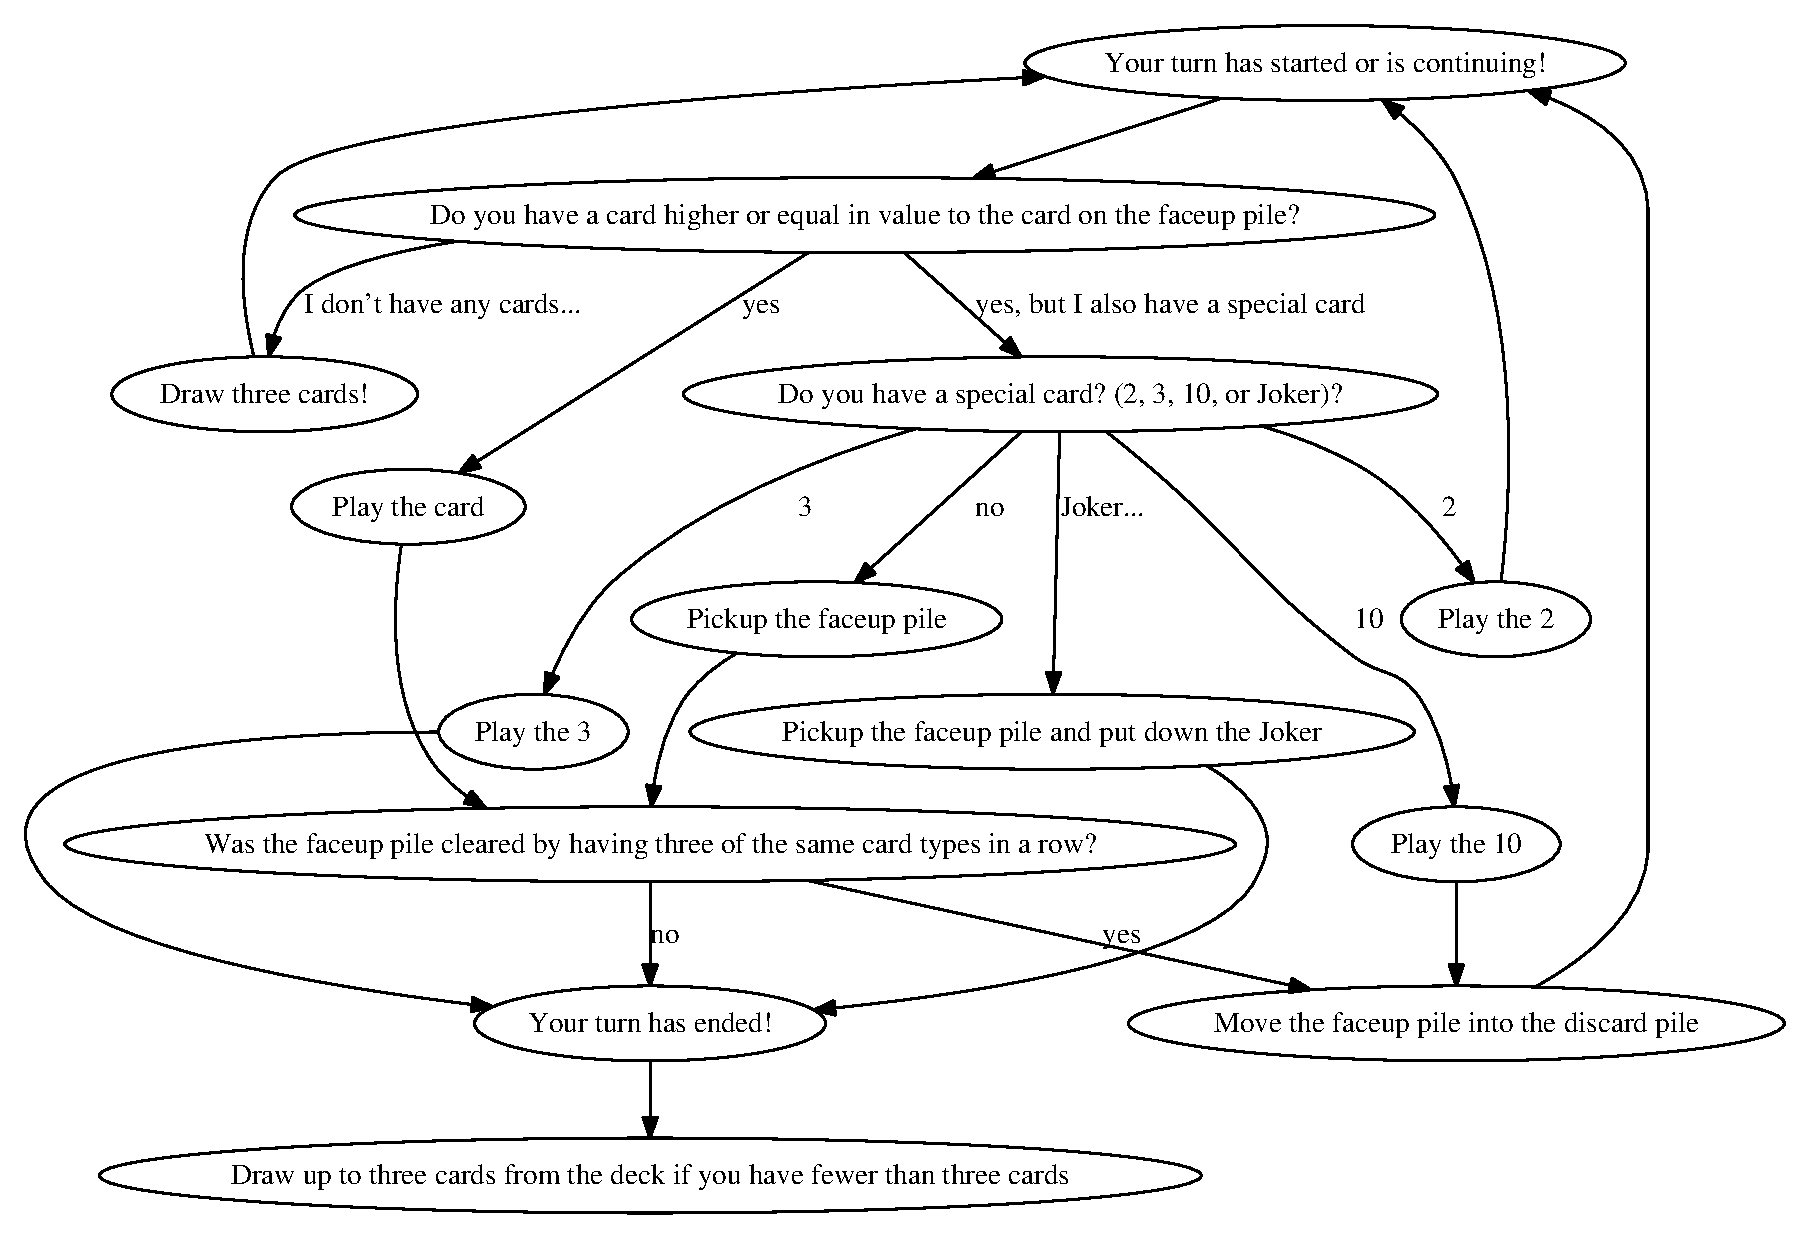
\includegraphics[width=6.5in]{Turns.eps}

If all cards have been picked up from the deck, follow the `End Game' rules for what cards to play next

\subsection*{End Game}
The end game starts when the all cards from the deck have been drawn. After that, when a player runs out of cards in hand they resort to the three cards that were placed face up at the start of the game. Once all the faceup cards are played and there are no more cards in hand, then a face down card is chosen at random and played. If the card does not `beat' the current card in the faceup pile, the faceup pile is moved into the players hand and continues from there.

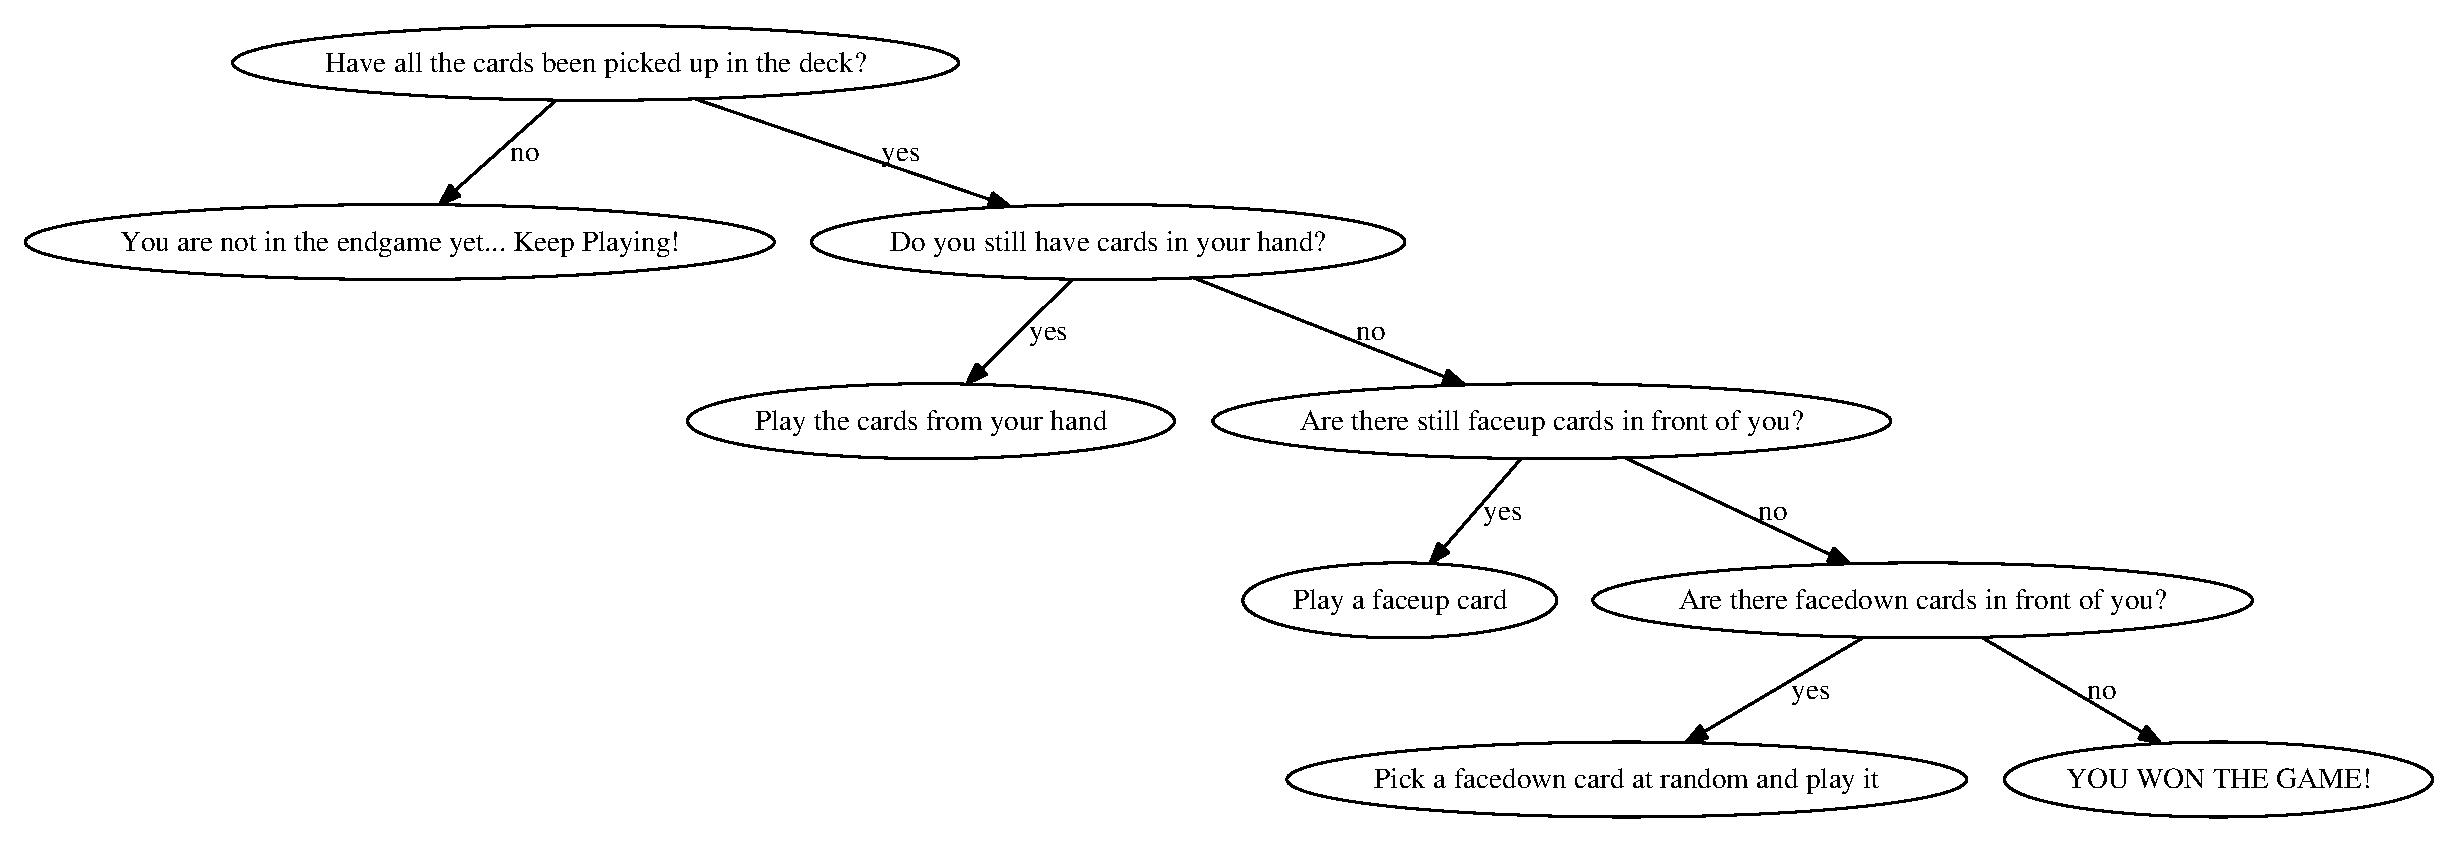
\includegraphics[width=6.5in]{Endgame.eps}

\subsection*{Winning}
The game is won, once a player has gotten rid of all their cards.

\end{document}